%
% Documento: Disposições
%

\chapter{Implementação}

    Neste capítulo irei abordar as tecnologias de utilizadas para a codificação do framework,
    os modulos e suas classes expostas para o usuario.


\section{Tecnologias Utilizadas}

    Para o desenvolvimento do framework foi utilizado apenas como linguagem para desenvolvimento o Python
    e para a manipulação e integração com o browser a biblioteca em python do Selenium Webdriver. Por ser um
    projeto que visa ser o mais simples e leve possivel apenas os modulos padrões do python estão sendo utilizado
    para o desenvolvimento desta ferramenta.


    \subsection{Python}

        Python \ref{swaroop2003byte} trata-se de uma linguagem de programação fácil de aprender e poderosa.
        Possui estruturas dados de alto nível e uma abordagem simples, mas eficaz, para a programação orientada
        a objetos. Com uma Sintaxe elegante e tipagem dinâmica, juntamente com uma interpretação natural, tornam
        a linguagem ideal para criação de scripts e desenvolvimento de aplicativos em muitas áreas nas maiorias das plataformas.

    \subsection{Selenium WebDriver}
        Falar Sobre Selenium Webdriver
    \subsection{GitHub}
        Falar Sobre Selenium Webdriver

\section{Modulos}

    O framework consiste em alguns modulos basicos, cada um com suas devidas utilidades e funções.
    A separação dos modulos foi dada com base em suas caracteristicas e funcionalidades.

    \begin{figure}[H]
        \vspace*{0,3cm}
        \centering
        \caption{Diagrama de Componentes}
        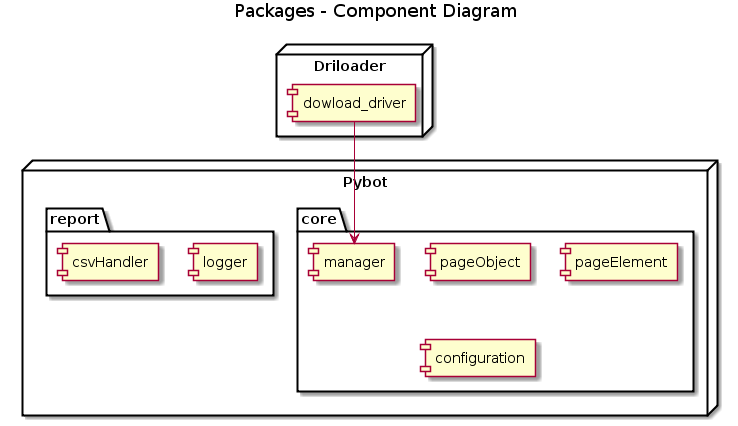
\includegraphics[width=1\textwidth]{./04-figuras/model}
        \label{fig:modules}
    \end{figure}

    \subsection{Core}
        \subsubsection{Manager}
        \subsubsection{Configuration}

    \subsection{Component}


        \subsubsection{WebElement}
        \subsubsection{PageObject}
        \subsubsection{PageElement}

    \subsection{Report}

        Estes modulo está destinado para geração de logs de execuções internas do framework, criação e controle
        de logs definidos pelos usuario e a criação de planilhas análiticas de dados extraidos das paginas.

        \subsubsection{Logger}
        \subsubsection{CsvHandler}
